\subsection{PESOS E RESTRIÇÕES}
\label{subsec:pesos_e_restricoes}

Apesar da importância da resolução de conflitos, existem diversas outras nuances durante o planejamento das grades horárias que precisam ser levadas em conta para que as grades produzidas sejam aplicáveis na prática.

\citeonline{ABRAMSON} sugere uma forma de permitir a otimização de múltiplas características simultanemente utilizando: uma função de custo ponderado. Esta função foi implementada, utilizando-se um sistema de métricas, cada qual mensura quantitativamente determinada característica da grade horária, e contém um peso que define a sua importância para a grade como um todo. 

A função de custo ponderado retorna um valor que representa a qualidade geral de uma grade horária, através do cálculo da média ponderada de todas as métricas de qualidade. Em outras palavras, quanto menor o custo, melhor a solução encontrada.

Adicionalmente, as métricas foram implementadas de forma que pudessem ser rígidas ou suaves. As métricas rígidas precisam ser perfeitamente atendidas para que a grade horária seja considerada viável, enquanto as métricas suaves promovem a melhoria da qualidade, mas não necessariamente precisam ser perfeitamente atendidas.

As próximas seções terão como objetivo explicar cada uma destas métricas e os desafios associados. A \autoref{subsec:salvamento} entrará em mais detalhes sobre como as grades horárias passaram a ser salvas após a implementação das métricas.

\subsubsection{Agrupamento de aulas}

Observando grades horárias escolares existentes, é possível notar que existe uma motivação para realizar agrupamentos, formando aulas duplas. Isso aumenta a produtividade das aulas, à medida que diminui trocas e deslocamento de professores entre as salas. Para produzir estes agrupamentos, foram adicionadas algumas métricas que fazem o otimizador penalizar:

\begin{enumerate}
	\item Aulas separadas;
	\item Aulas desagrupadas;
	\item Excessos de aulas iguais para determinada turma em um dia;
	\item Dias com todas aulas planejadas distintas para deteriminada turma;
\end{enumerate}

Para contextualizar estas situações, a seguir serão apresentados alguns quadros.

\begin{quadro}[!htb]
	\centering
	\caption{Exemplo de dia com aulas separadas.\label{qua:aulasSeparadas}}
	\begin{tabular}{|p{3cm}|p{3cm}|p{3cm}|}
		\hline
		\textbf{Aula} & \textbf{Professor} & \textbf{Matéria} \\
		\hline
		1 & Marcos & Matemática \\
		\hline
		2 & Fábio & Física \\
		\hline
		3 & Marcos & Matemática \\
		\hline
		4 & Luciana & Português \\
		\hline
		5 & Luciana & Português \\
		\hline
		6 & Luciana & Português \\
		\hline
	\end{tabular}
	\fonte{Autoria própria}
\end{quadro}
\pagebreak

Observando o quadro \ref{qua:aulasSeparadas}, é possível notar:

\begin{itemize}
	\item Aulas separadas: 1, 2 e 3, visto que não estão em nenhum agrupamento;
	\item Aulas desagrupadas: 1 e 3, pois consistem em múltiplas aulas iguais, no mesmo dia, que não foram agrupadas;
	\item Excessos de aulas: 4, 5, 6, pois consiste em uma aula tripla, algo considerado não desejável neste trabalho
\end{itemize}`

Por fim, a situação de dias com todas aulas diferentes, que serão referidos como ``Dias fragmentados'' neste trabalho, pode ser observada no quadro \ref{qua:fragmentado}.

\begin{quadro}[!htb]
	\centering
	\caption{Exemplo de dia fragmentado.\label{qua:fragmentado}}
	\begin{tabular}{|p{3cm}|p{3cm}|p{3cm}|}
		\hline
		\textbf{Aula} & \textbf{Professor} & \textbf{Matéria} \\
		\hline
		1 & Marcos & Matemática \\
		\hline
		2 & Fábio & Física \\
		\hline
		3 & Luciana & Português \\
		\hline
		4 & Roberto & Geografia \\
		\hline
		5 & Renato & História \\
		\hline
	\end{tabular}
	\fonte{Autoria própria}
\end{quadro}

\subsubsection{Constantes}

Durante o desenvolvimento, concebeu-se o conceito de ``Aulas constantes'', como aulas que absolutamente devem ser alocadas em determinada posição da grade horária. Isto é útil para guiar o otimizador rumo a uma solução desejada, quando já são conhecidas algumas aulas que devem ser fixas. 

Como exemplo de caso de uso, uma escola com seis aulas diárias pode ter alguns dias da semana com menos aulas, e pode ser interessante definir explicitamente quais dias devem ter a última aula da grade horária não alocada (vazia). A figura \ref{fig:constantes} mostra um exemplo de configuração de aulas constantes para determinada grade horária.

\begin{figure}[!htb]
	\centering
	\caption{Aulas constantes}
	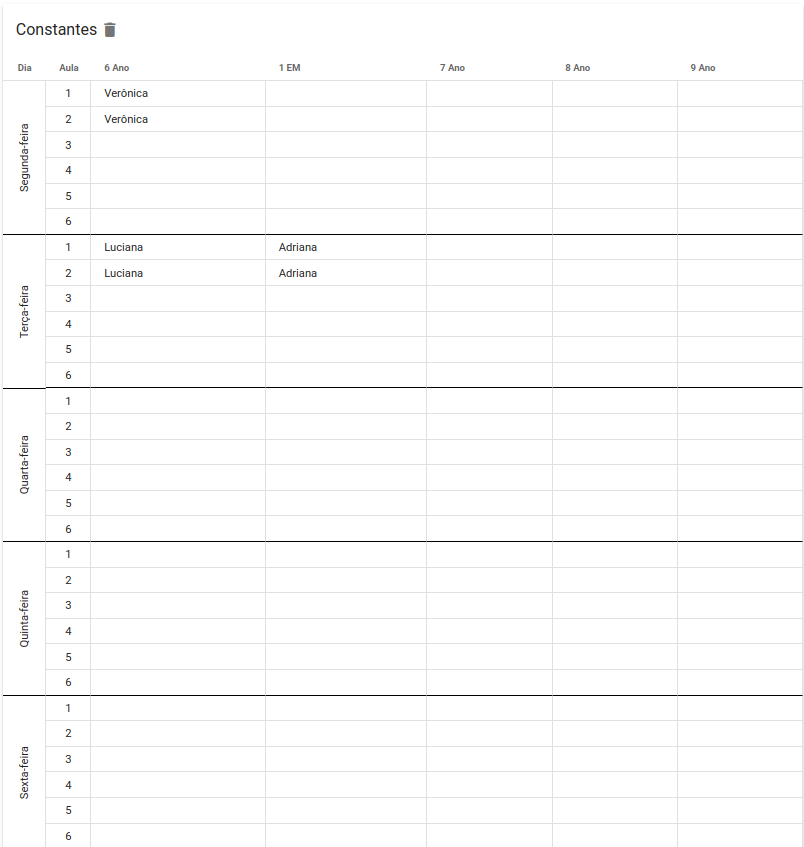
\includegraphics[width=1\textwidth]{./dados/figuras/constantes}
	\fonte{Autor}
	\label{fig:constantes}
\end{figure}
\pagebreak

Considerando a natureza absoluta das aulas constantes, estas não são consideradas um métrica de qualidade, e não possuem um peso próprio. Em vez disso, no método ``GeraGradeInicial'' do algoritmo \ref{alg:otimizadorInicial}, o otimizador já aloca as aulas constantes nas posições desejadas, e a função ``EscolheHorariosAleatoriosValidos'' não seleciona posições que estejam alocadas com aulas constantes. Desta forma, um vez que as aulas constantes são posicionadas na grade horária, estas nunca são movidas durante os passos de otimização.

\subsubsection{Restrições}

As restrições representam o oposto das aulas constantes: posições em que determinadas aulas não devem ser alocadas. Implementaram-se no otimizador restrições suaves e rígidas, cada uma podendo também receber um peso customizado. Dessa forma, é possível configurar o otimizador para nunca alocar determinada aula em certa posição da grade, ou apenas evitar isso.

Como exemplo de uso dessa funcionalidade, a figura \ref{fig:restricoes} demonstra uma configuração de restrições para determinado professor que não pode ser alocado nas duas últimas aulas de qualquer dia da grade horária.

\begin{figure}[!htb]
	\centering
	\caption{Restrições}
	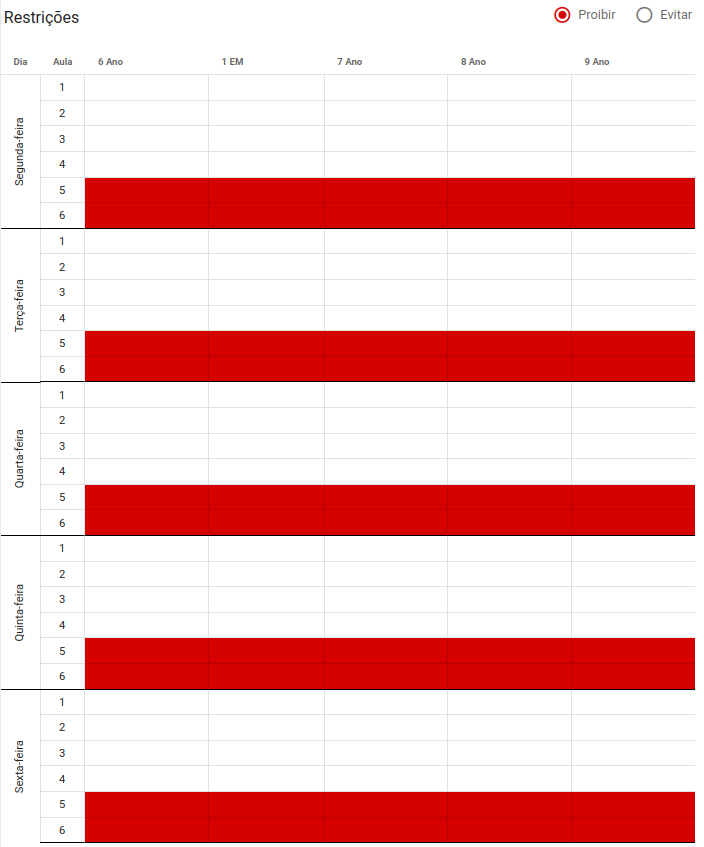
\includegraphics[width=1\textwidth]{./dados/figuras/restricoes}
	\fonte{Autor}
	\label{fig:restricoes}
\end{figure}
\pagebreak

No caso das restrições, a métrica associada mensura a quantidade de restrições violadas, ou seja, posições em que determinada aula foi alocada, mas não deveria ter sido.

\subsubsection{Limite de dias trabalhados}

Adicionou-se esta métrica como uma forma de especificar um número máximo de dias por semana em que um professor pode ser alocado. Como exemplo de aplicação dessa configuração, considere uma grade horária que comporta 30 horários de aulas (6 aulas por dia, 5 dias por semana, por exemplo). Se um professor deve minstrar 15 aulas nessa grade, o ideal é que suas aulas sejam concentradas em apenas três dias. Logo, configurando-se um limite de 3 dias de trabalho para esse professor, asseguramos que suas aulas serão alocadas de uma forma mais compacta na grade horária.

Esta métrica simplesmente mensura o excesso de dias trabalhados, conforme os limites configurados. Por exemplo, se determinado professor tem um limite de 2 dias trabalhados, mas teve aulas alocadas em quatro dias diferentes, a métrica considera um desvio de dois dias.


\subsubsection{Regiões}

O conceito de regiões foi concebido como uma forma de proporcionar ainda mais controle ao usuário, sobre o posicionamento das aulas na grade horária. Cada região consiste em um grupo arbitrário de posições da grade horária, associado a uma regra relacionada a uma quantidade de aulas. Com as regiões, é possível determinar mínimos, máximos ou quantidades exatas de aulas que devem ser alocadas em certas posições da grade horária.

Como exemplo de uso das regiões, a figura \ref{fig:regioes} demonstra uma configuração utilizada para assegurar que em todos os dias da grade horária, o professor tenha alguma aula alocada no primeiro horário.

\begin{figure}[!htb]
	\centering
	\caption{Exemplo de região}
	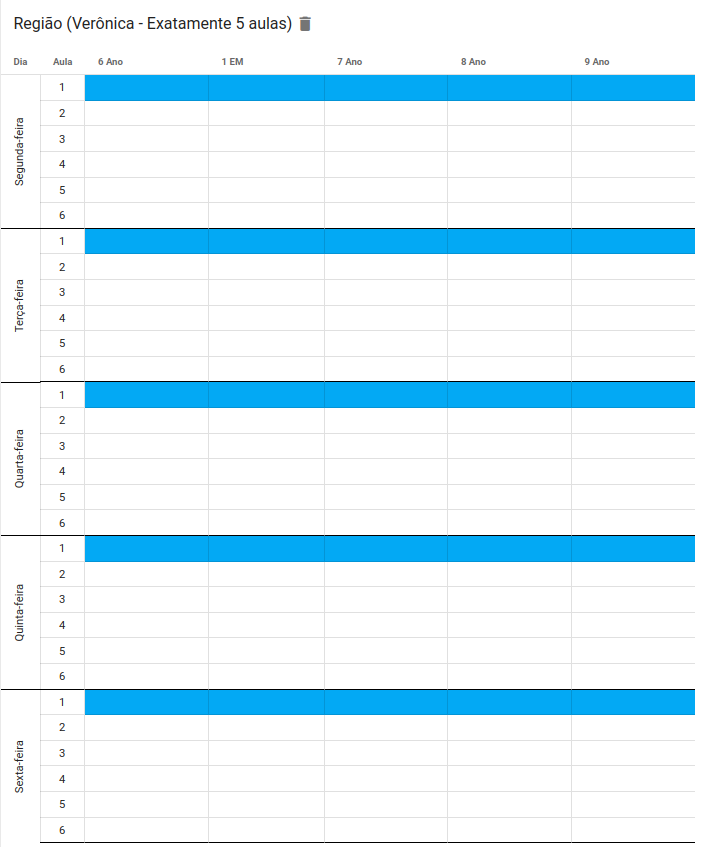
\includegraphics[width=1\textwidth]{./dados/figuras/regioes}
	\fonte{Autor}
	\label{fig:regioes}
\end{figure}
\pagebreak

A região configurada na \ref{fig:regioes} pode ser interpretada da seguinte forma: a professora ``Verônica'' deve ter exatamente cinco aulas alocadas dentro das posições marcadas pela cor azul. Como o otimizador não permite conflitos, cada uma das cinco aulas deverá ser alocada em um dos diferentes dias, garantindo que a professora terá uma aula agendada no primeiro horário de cada um dos dias.

Neste caso, a métrica associada mensura o erro das regiões, ou seja, a diferença entre a quantidade de aulas esperada de acordo com a regra de cada região e a quantidade real de aulas alocadas.

\subsubsection{Grupos de Alinhamento}

Os grupos de alinhamento representam uma forma de configurar o otimizador para agendar aulas para diferentes turmas, nos mesmos horários. Isto é útil para atender a restrições relacionadas ao conceito dos Itinrários Formativos do Novo Ensino Médio, conforme citado na \autoref{sec:novo_ensino_medio}.

Como exemplo de utilização dos grupos de alinhamentos, tem-se a configuração da figura \ref{fig:gruposAlinhamento}.

\begin{figure}[!htb]
	\centering
	\caption{Exemplo de grupo de alinhamento sobre a grade horária gerada}
	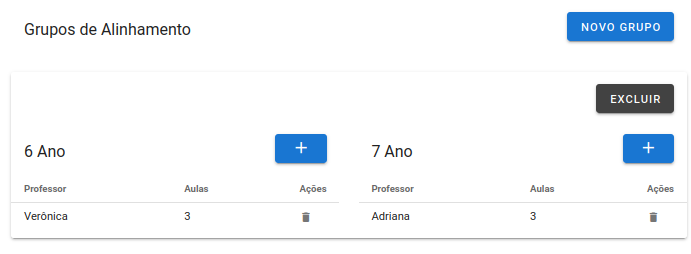
\includegraphics[width=1\textwidth]{./dados/figuras/gruposAlinhamento}
	\fonte{Autor}
	\label{fig:gruposAlinhamento}
\end{figure}
\pagebreak

O efeito da configuração do grupo de alinhamento da figura \ref{fig:gruposAlinhamento}, pode ser observado na grade horária final gerada na figura \ref{fig:alinhados}, com as aulas corretamente alocadas em horários simultâneos.

\begin{figure}[!htb]
	\centering
	\caption{Efeito de grupo de alinhamento}
	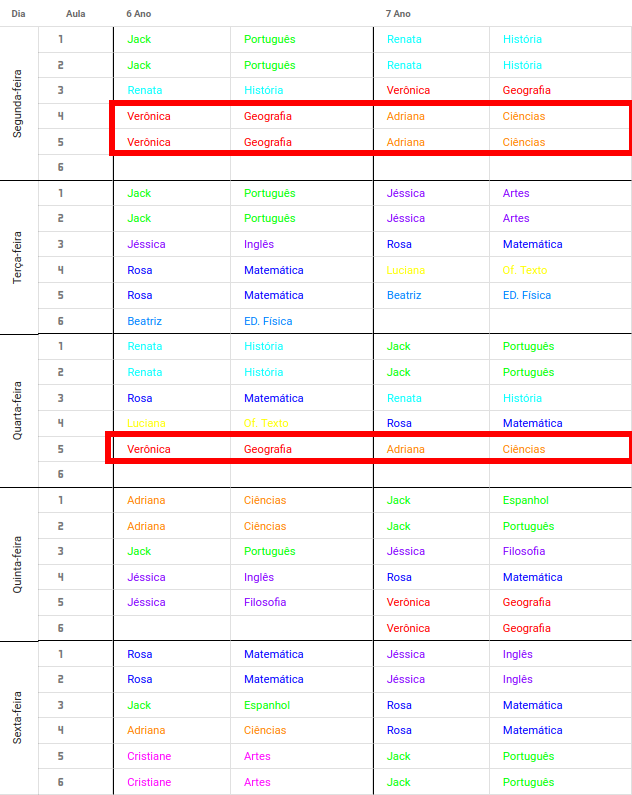
\includegraphics[width=1\textwidth]{./dados/figuras/alinhados}
	\fonte{Autor}
	\label{fig:alinhados}
\end{figure}
\pagebreak

Implementaram-se duas métricas de qualidade relacionadas aos grupos de alinhamento, uma que mensura a quantidade de grupos formados e a quantidade de aulas ``desalinhadas'', ou seja, aulas que deveriam ser agendadas no mesmo horário, mas que não foram.

No caso da figura \ref{fig:alinhados}, foram formados dois grupos (demarcados em vermelho), e nenhuma aula ficou desalinhada, ou seja, todas as seis aulas configuradas no grupo de alinhamento foram corretamente alocadas em horários simultâneos.

\subsubsection{Janelas}

As janelas consistem em situações em que a jornada de trabalho de determinado professor apresenta um horário sem aulas alocadas, fazendo com que o docente fique ocioso. O quadro \ref{qua:janelas} exemplifica esta situação.

\begin{quadro}[!htb]
	\centering
	\caption{Exemplo de dia com janela.\label{qua:janelas}}
	\begin{tabular}{|p{3cm}|p{3cm}|p{3cm}|p{3cm}|}
		\hline
		\textbf{Aula} & \textbf{6ºAno} & \textbf{7ºAno} & \textbf{8ºAno} \\
		\hline
		1 & Jéssica & Rosa & Adriana \\
		\hline
		2 & Jéssica & Rosa & Adriana \\
		\hline
		3 & Fábio & Jéssica & Rosa \\
		\hline
		4 & Adriana & Jéssica & Rosa \\
		\hline
		5 & Beatriz & Adriana & Jéssica \\
		\hline
	\end{tabular}
	\fonte{Autoria própria}
\end{quadro}

No quadro \ref{qua:janelas}, a professora Adriana tem uma janela na terceira aula, visto que tem aulas alocadas antes e depois (aulas 1, 2, 4 e 5). Em contrapartida, apesar de não ter nenhuma aula planejada no quinto horário, Rosa não tem janelas neste exemplo, pois pode encerrar sua jornada de trabalho na quarta aula.

A métrica de janelas mensura o número de horários na grade que apresentam estes horários ociosos, para cada professor.

\subsubsection{Preferências}

As preferências consistem em configurações que informam ao otimizador características preferíveis para a alocação das aulas de cada professor. Implementaram-se os seguintes tipos de preferência no otimizador:

\begin{enumerate}
	\item Preferência de primeiras aulas;
	\item Preferência de últimas aulas;
	\item Preferência específica de última aula
\end{enumerate}

\begin{figure}[!htb]
	\centering
	\caption{Configuração de preferências}
	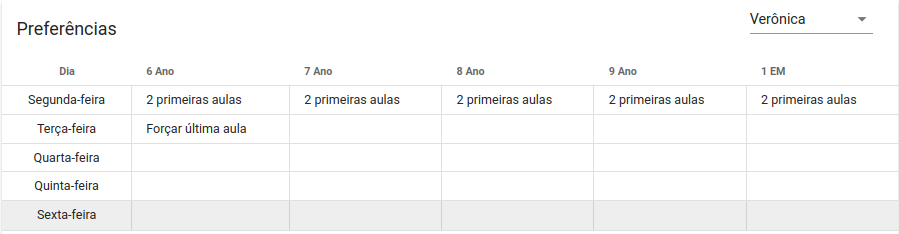
\includegraphics[width=1\textwidth]{./dados/figuras/preferencias}
	\fonte{Autor}
	\label{fig:preferencias}
\end{figure}

A \autoref{fig:preferencias} representa um exemplo de configuração de preferências para determinado professor. Neste caso, a configuração informa ao otimizador que na segunda-feira, as aulas de ``Verônica'' devem ser alocadas desde o início do dia, não ultrapassando um total de aulas; e que na turma do ``6º Ano'', caso haja uma aula dessa professora, esta deve ser alocada na última aula.

Vale ressaltar que o diferencial da preferência específica de última aula é que esta considera a possibilidade de aulas vazias, ou seja, caso o último horário do dia não tenha uma aula alocada, a preferência considera que a aula deve ser alocada na penúltima aula.

\subsubsection{Mínimos e máximos}

Desenvolveram-se métricas de qualidade relacionadas a quantidades de aulas ministradas por dia. Como pode ser visto na figura \ref{fig:tela_minimos}, estas métricas permitem configurar quantidades mínimas e máximas de aulas por dia para cada professor.

\begin{figure}[htb!]
	\centering
	\caption{Mínimos de aulas configuradas na interface}
	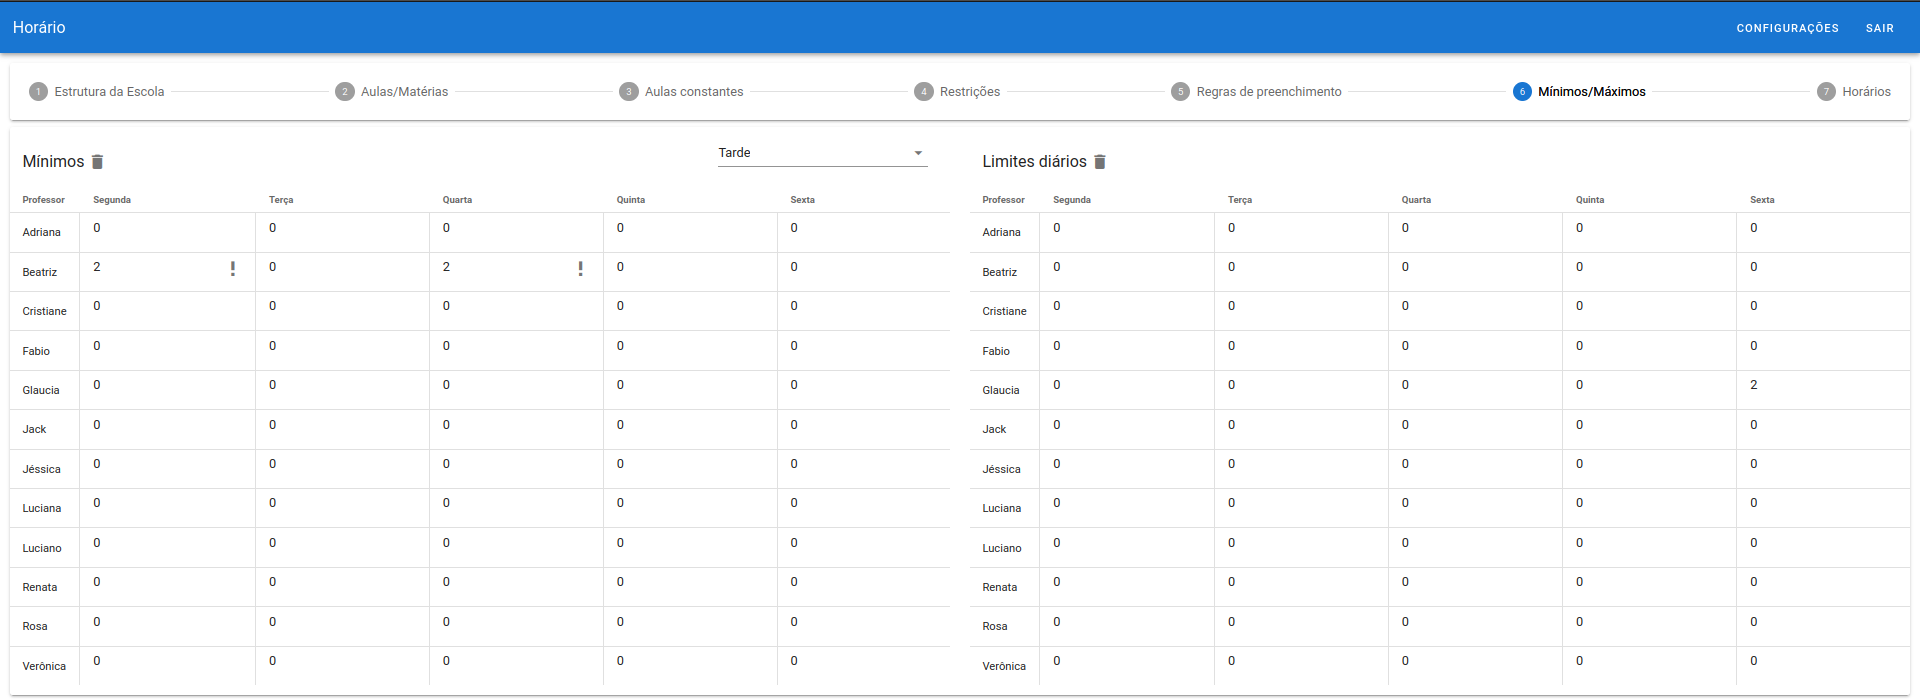
\includegraphics[width=1\textwidth]{./dados/figuras/minimos_configurados}
	\fonte{Autor}
	\label{fig:tela_minimos}
\end{figure}

O cálculo das métricas de qualidade relacionadas aos mínimos e máximos consiste no cálculo do erro, ou seja a quantidade de aulas alocada subtraída da quantidade de aulas esperada. Vale ressaltar que enquanto os mínimos são configuráveis por turno, os máximos são interpretados como limites diários, e consequentemente levam em conta a soma da quantidade de aulas em todos os turnos. Por exemplo, se um professor tem um limite diário de cinco aulas configurado, a soma de suas aulas naquele dia, em todos os turnos, não deverá ultrapassar cinco.

\subsubsection{Armazenamento de soluções}
\label{subsec:salvamento}

Com a adição das métricas, o critério para considerar uma grade horária como uma solução válida ficou mais estrito, e em muitos casos tornou-se impossível obter uma grade que atenda perfeitamente todas as nuances. Tendo isto em mente, foi necessário implementar uma funciondalide de armazenamento de grades horárias um pouco mais detalhada. O resultado disso, pode ser visto no algoritmo \ref{alg:otimizadorComRestricoes}.

\begin{algorithm}
	\caption{Otimizador com persistência de grades horárias}
	\label{alg:otimizadorComRestricoes}
	\KwIn{Lista de professores $LP$, lista de turmas $LT$, matriz de aulas por professor por turma $MA$, temperatura inicial $TI$, Taxa de resfriamento $TR$}
	\KwOut{Grade horária de professores otimizada}
	$temperatura \leftarrow TI$\\
	$grade \leftarrow$ CriaGradeInicial$(LP, LT, MA)$\\
	$iteracoesSemAlteracao \leftarrow 0$\\
	$solucoes \leftarrow$ lista vazia\\
	\While {condição de parada não atingida} {
		$deltaTotal \leftarrow 0$\\
		\For {$passo = 0$ até $numeroPassos$} {
			$turma \leftarrow grade.EscolheTurmaAleatoria()$\\
			$linhas \leftarrow grade.EscolheHorariosAleatoriosValidos(sala)$\\
			$delta \leftarrow grade.CalculaDelta(sala, linhas)$\\
			$probabilidade \leftarrow e^{-delta/temperatura}$\\
			$valorAceite \leftarrow Aleatorio(0, 1)$\\
			\If {$delta < 0$ ou $probabilidade \ge valorAceite$} {
				$grade.PermutaProfessores(sala, linha1, linha2)$\\
				$deltaTotal \leftarrow deltaTotal + delta$\\
				\If {grade não existe na lista de soluções} {
					insere grade na lista de soluções\\
					limita lista de soluções às 100 melhores grades\\
				}
			}
		}
		\eIf {$delta = 0$} {
			$iteracoesSemAlteracao \leftarrow iteracoesSemAlteracao + 1$\\
		}{
			$iteracoesSemAlteracao \leftarrow 0$\\
		}
		\If {$iteracoesSemAlteracao \ge 15$} {
			salvaGradesRelevantes()\\
			apaga lista de soluções\\
			$temperatura \leftarrow TI$\\
			$iteracoesSemAlteracao \leftarrow 0$\\
		}
		$temperatura \leftarrow temperatura * TR$
	}
\end{algorithm}
\pagebreak

Consinderando as diversas métricas de qualidade que as grades horárias passaram a ter, o método ``salvaGradesRelevantes'' do algoritmo \ref{alg:otimizadorComRestricoes} salva, para cada métrica escolhida, as 5 grades que tiveram a melhor pontuação em cada métrica. A princípio, optou-se por utilizar as métricas de qualidade geral (média ponderada de todas as métricas), janelas, agrupamento de aulas e número de preferências resolvidas, mas este método pode ser expandido para qualquer uma das métricas implementadas no sistema.

Devido à complexidade do problema e à natureza não determinística do algoritmo aplicando \textit{Simulated Annealing}, é necessário utilizar o laço de repetição no presente no algoritmo \ref{alg:otimizadorComRestricoes}, controlado pela condição de parada. Em um cenário de produção, poderia ser utilizada como condição de parada um intervalo de tempo máximo de execução, ou um limite de soluções gerado.

O principal desafio no desenvolvimento deste incremento foi manter a função ``CalculaDelta'' performática, já que esta é executada a cada passo de otimização. Para garantir uma performance aceitável, a função precisou ser implementada de forma que a variação de custo fosse calculada sem necessitar efetivamente a troca das aulas. Em outras palavras, a implementação simples, que seria realizar a permutação das aulas, calcular o custo e comparar com o custo atual da solução para obter a variação e depois desfazer a troca, seria ineficiente demais.
